%%%%%%%%%%%%%%%%%%%%%%%%%%%%%%%%%%%%%%%%%%%%%%%%%%%%%%%%%%%%%%%%%%%%%%%%%%%%
%% Trim Size: 9.75in x 6.5in
%% Text Area: 8in (include Runningheads) x 5in
%% ws-mpla.tex   :   29-9-2008
%% TeX file to use with ws-mpla.cls written in Latex2E.
%% The content, structure, format and layout of this style file is the
%% property of World Scientific Publishing Co. Pte. Ltd.
%% Copyright 1995, 2002 by World Scientific Publishing Co.
%% All rights are reserved.
%%%%%%%%%%%%%%%%%%%%%%%%%%%%%%%%%%%%%%%%%%%%%%%%%%%%%%%%%%%%%%%%%%%%%%%%%%%%
%%

\documentclass{ws-mpla}
\usepackage[super]{cite}
\usepackage{graphicx}
\usepackage{booktabs}% http://ctan.org/pkg/booktabs
\usepackage{multirow}% http://ctan.org/pkg/multirow
\begin{document}

\markboth{Michael Helland}
{Hubble's Law as Photon Velocity}

%%%%%%%%%%%%%%%%%%%%% Publisher's Area please ignore %%%%%%%%%%%%%%
\catchline{}{}{}{}{}
%%%%%%%%%%%%%%%%%%%%%%%%%%%%%%%%%%%%%%%%%%%%%%%%%%%%%%%%%%%%%%%%%%%

\title{HUBBLE'S LAW AS PHOTON VELOCITY}

\author{\footnotesize MICHAEL HELLAND}

\address{Seattle, WA 98134,
United States\\
mike@mikehelland.com}


\maketitle

\pub{Received (Day Month Year)}{Revised (Day Month Year)}

\begin{abstract}
Applied directly to the wave speed formula, cosmological redshifts suggest a photon`s velocity decreases with distance from its source. 
When examined, computer models with photons in static space that decelerate according to Hubble`s constant are shown to produce the observed 
z values relative to distance. The duration of the photon`s journey to its destination increases 
as it decelerates, which mostly correlates to the expected co-moving distance of the standard model, deviating from the 
standard model by predicting a slower increase in redshifts over time when $z > 8.0$, eliminating the need for Hubble`s 
constant to change with time. 

\keywords{redshift; Hubble's Law; photon.}
\end{abstract}

\ccode{PACS Nos.: 02.70.−c, 07.05.Tp, 14.70.Bh, 98.80.Es, 98.62.Py}

\section{Introduction}	

Finding the right value for Hubble's constant has been difficult.\cite{Riess}\cite{Planck} To examine the problem, let's start with a simple JavaScript model of a photon
traveling through space. 

\begin{verbatim}
    simple = {
        photon: {d: 0},
        next: function () {
            this.photon.d += c
        }
    }
\end{verbatim}

The simple model contains two things, a photon and a next() function. The photon has a distance $d$ which starts at zero. 
Every time next() is called, $d$ increases by $c$. In this model, units of distance are in Mly (million light years) and units of time are in million years. 
That makes $c = 1$, to keep things simple.

We're going to give the photon a series of targets to pass by, each target 200 Mly apart, and we will record the time and distance when a target is passed. Here's that program:

\begin{verbatim}
// the speed of light, 1 Mly / million years
const c = 1

function run(model) {

    // create targets 200 million light years apart
    model.targets = []
    for (var i = 200; i <= 30000; i+=200) 
        model.targets.push({d: i})

    var t = 0
    var nextTarget = 0

    // start the loop
    while (model.targets[nextTarget]) {

        //advance the model 1 million years
        t += 1
        model.next()

        // if we hit a target record the time
        if (model.photon.d >= model.targets[nextTarget].d) {
            
            console.log("Target reached", t)
            model.targets[nextTarget].hitT = t
            model.targets[nextTarget].hitD = model.photon.d

            nextTarget += 1
        }
    }
}
\end{verbatim}

In this simple model, the photon will reach the first target at $t=200$, the second target at $t=400$ and so on.

Our universe, however, is not that simple. We observe cosmologically redshifted light, 
which is interpreted as the recessional velocity of the light source. That leads to a universe that expands.

In an expanding universe, the targets will be moving away from the photon's source according to Hubble's Law, $v = H \times D$, 
where $v$ is the velocity of the target, $H$ is Hubble's constant, and $D$ is the distance of the target.

To update our simple model to an expanding model, we just add some code to the next() function that loops through the targets and moves them 
according to Hubble's Law:

\begin{verbatim}
    expanding = {
        photon: {d: 0},
        next: function () {
            this.photon.d += c
    
            for (var target of this.targets)
                target.d += H * target.start
        }
    }
\end{verbatim}

While simple.next() just moves the photon, expanding.next() moves the photon and the targets. The important new line in this model 
(target.d  += H * target.start) contains a new constant, $H$, Hubble's constant. 
So what value do we use for $H$? According to observations of relatively near phenomena, $H$ is measured to be 74 km/sec/Mpc.\cite{Riess} 
But according to measurements at our most distant observable range, $H$ is measured as 67.4 km/sec/Mpc.\cite{Planck}
To use these values in the model, they must be converted to the proper units.

\begin{romanlist}
 \item convert (km/s/Mpc) to (km/s/Mly) 
 \item convert (km/s) to (light years / year) 
\end{romanlist}

Which gives: 

\begin{verbatim}
    74 km/s/Mpc = 22.688 km/s/Mly = 7.5679e-5 ly/y/Mly = 0.00076
    67 km/s/Mpc = 20.541 km/s/Mly = 6.8520e-5 ly/y/Mly = 0.00069
\end{verbatim}

When you run the expanding model, notice that the targets are moving away from the photon's source. The first one ($H=0.00076$) 
expands slightly faster than the second one ($H=0.00069$). 

\begin{figure}[h]
\centerline{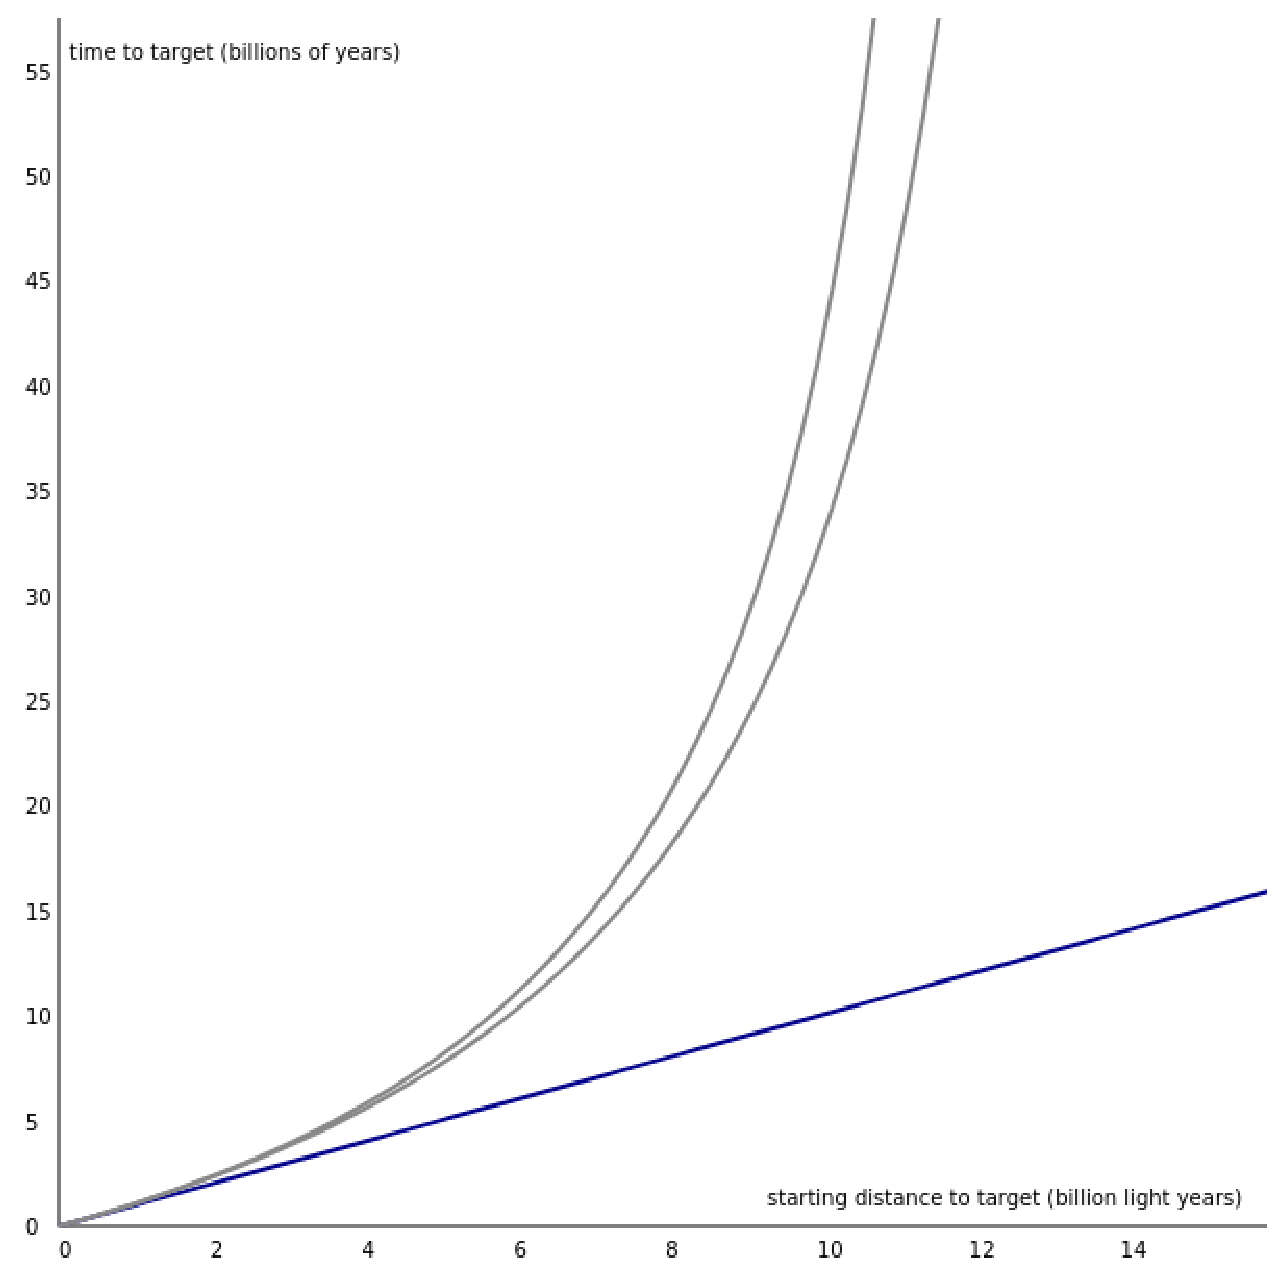
\includegraphics[width=2.1in]{graph_white_expanding.eps}}
\vspace*{8pt}
\caption{Photons in an expanding universe (gray) reach targets at an increasing rate compared to a static universe (blue)}
\label{fig:expanding}
\end{figure}

As the targets recede, the time $t$ it takes the photon to reach the next target increases, as can be seen by the gray lines in Figure \ref{fig:expanding} 
shooting up and away from the blue line of the simple model.

The difference in the values of $H$ may seem small, but to cosmologists it begs to be resolved.

\section{Hypothesis}

\begin{quote}
\emph{''We may state with some confidence that red-shifts are the familiar velocity-shifts, or else they represent some unrecognized principle of nature. 
We cannot assume that our knowledge of physical principles is yet complete; 
nevertheless, we should not replace a known, familiar principle by an ad hoc explanation unless we are forced to that step by actual observations.''}
E. Hubble, Ref. 3
\end{quote}



Edwin Hubble said that it was convenient for the redshift to be interpreted as a Doppler-like effect, leading to the expanding universe theory. He also said redshifts might be interpreted as how nature actually works. In other words, the redshifts aren't caused by some other phenomenon; cosmological redshift is a new phenomenon in-and-of itself. However, he cautioned, if there are existing ways to explain the redshifts, adding a new principle of nature should be avoided.

But choosing the path of the familiar principles over a new principle has forced us to propose several new principles anyways, including dark energy and inflation. 
It is also unclear, despite many precise measurements, how fast space is expanding.

Let's back up then and ask: if cosmological redshifts do represent a new principle of nature, what is that principle? Consider the following premises:

\begin{romanlist}
 \item a decrease in frequency is observed 
 \item the speed of a wave is v = frequency $\times$ wavelength 
\\
\\
Therefore, if these premises are taken literally and plainly (and a bit naively):
\\
%\begin{itemlist}
 \item the observed decrease in frequency should result in a decrease in speed
%\end{itemlist}
\end{romanlist}

\subsection{Hypothesis 1}

To examine this literal interpretation of redshifts, let's make a new model where the speed of a photon begins at $c$ and 
decreases as the distance from its source increases. The simplest of these models is one where $H \times D$ is subtracted from $c$.

\begin{equation}
v_{photon} = c - H \times D
\end{equation}\\

Here is the hypothesis as code:\\

\begin{verbatim}
    hypothesis1 = {
        photon: {d: 0},
        next: function () {
            this.photon.d += c - H * this.photon.d
        }
    }
\end{verbatim}

Figure 2 shows its output with previous models:

\begin{figure}[h]
\centerline{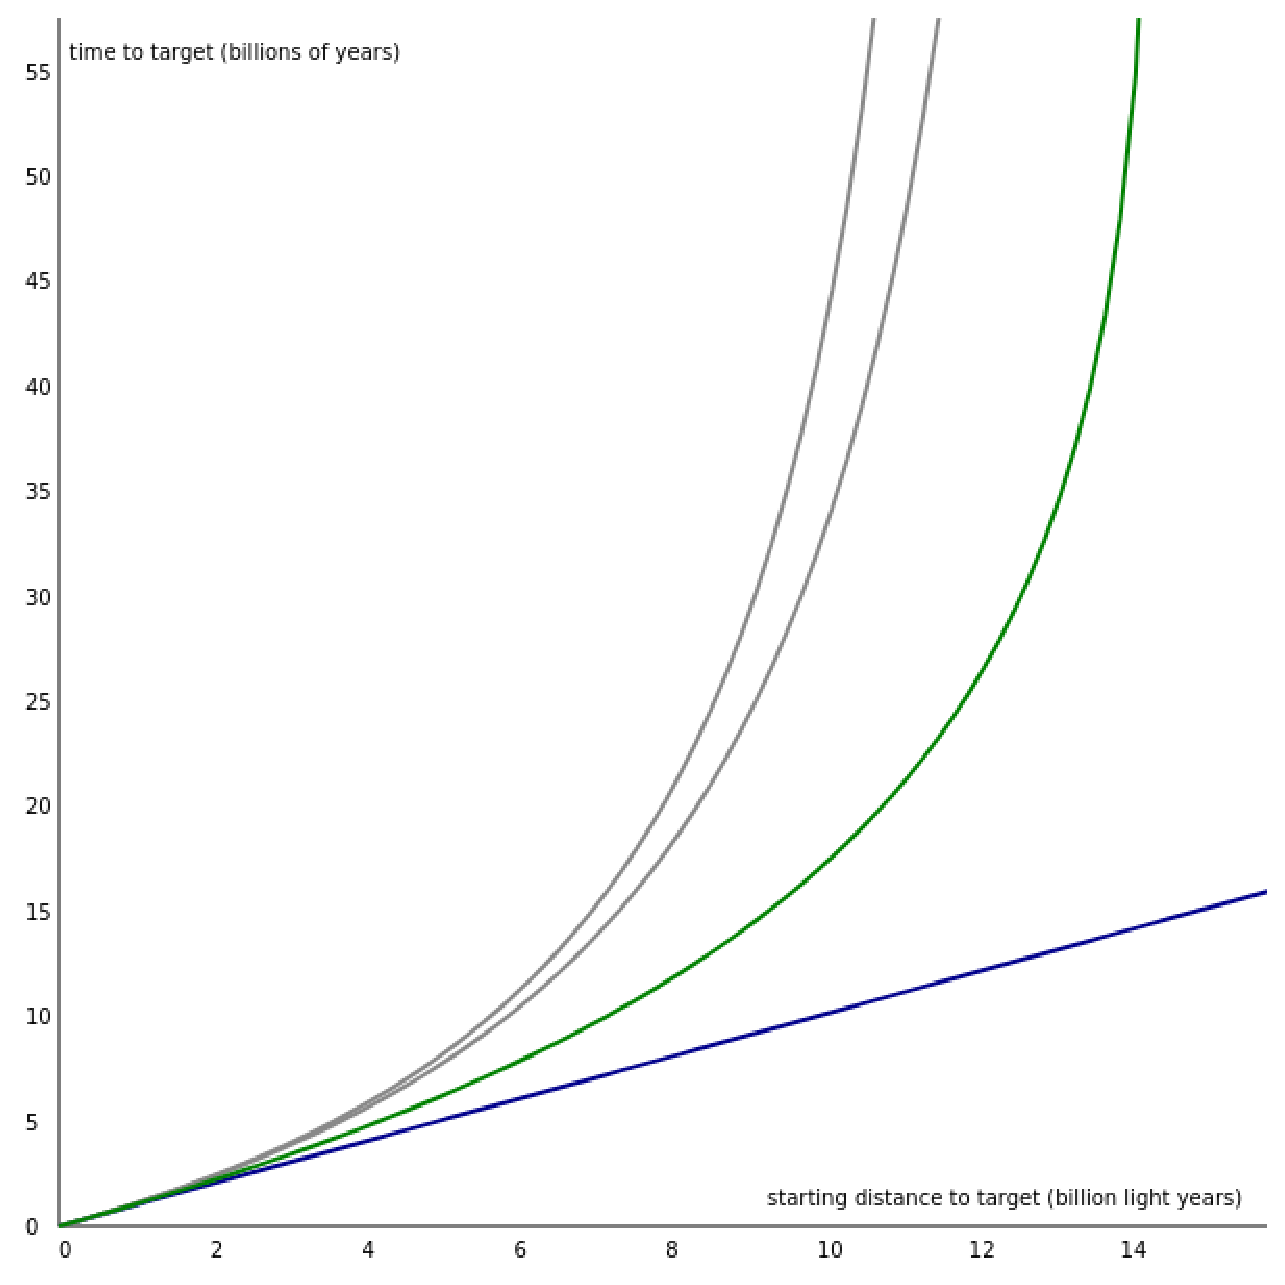
\includegraphics[width=4.0in]{graph_white_hypothesis1.eps}}
\vspace*{8pt}
\caption{Hypothesis 1 (green) predicts photons reach their targets after photons in a simple universe (blue) and before photons in an expanding universe (gray)}
\label{fig:hypothesis1}
\end{figure}


This hypothesis achieves something interesting. Even though the targets are stationary, the time it takes to reach the next target increases in a way that is similar to, but not exactly, the time it would take to reach a moving target.
The difference between the expanding model and hypothesis 1 is that $H \times D$ has been moved from the velocity of the targets, to the velocity of the photon.

\subsection{Frequency check}

Let's check to see how this affects frequency and redshift. We're going to modify $hypothesis1$, not to do anything different, but to log more data. 
We'll store the photon's velocity as $v$. We'll give the photon an initial wavelength $w$ and frequency $f_{emitted}$ of 499.65 nm and $6\times 10^5$  Ghz. 
Then we'll calculate a new frequency $f$ based on the photon's new velocity $v$.

\begin{verbatim}
  hypothesis1 = {
      photon: {d: 0, f_emitted: 6e5, w: 499.65},
      next: function () {
          this.photon.v = c - H * this.photon.d
          this.photon.d += this.photon.v
  
          this.photon.f = this.photon.v * 299792458 / this.photon.w
      }
  }
\end{verbatim}

Knowing the initial frequency and new frequency allows us to calculate z using the z frequency formula:

\begin{equation}
z = \frac{f_{emitted} - f_{observed}}{f_{observed}}
\end{equation}

Now we can update the run() function to log the photon's velocity, frequency, and z at the time it reaches a target.

\begin{verbatim}
  console.log("Target reached", t)
  targets[nextTarget].hit = t
  targets[nextTarget].v = photon.v
  targets[nextTarget].f = photon.f
  targets[nextTarget].z = (photon.f_emitted - photon.f) / photon.f
\end{verbatim}

\begin{figure}[p]
\centerline{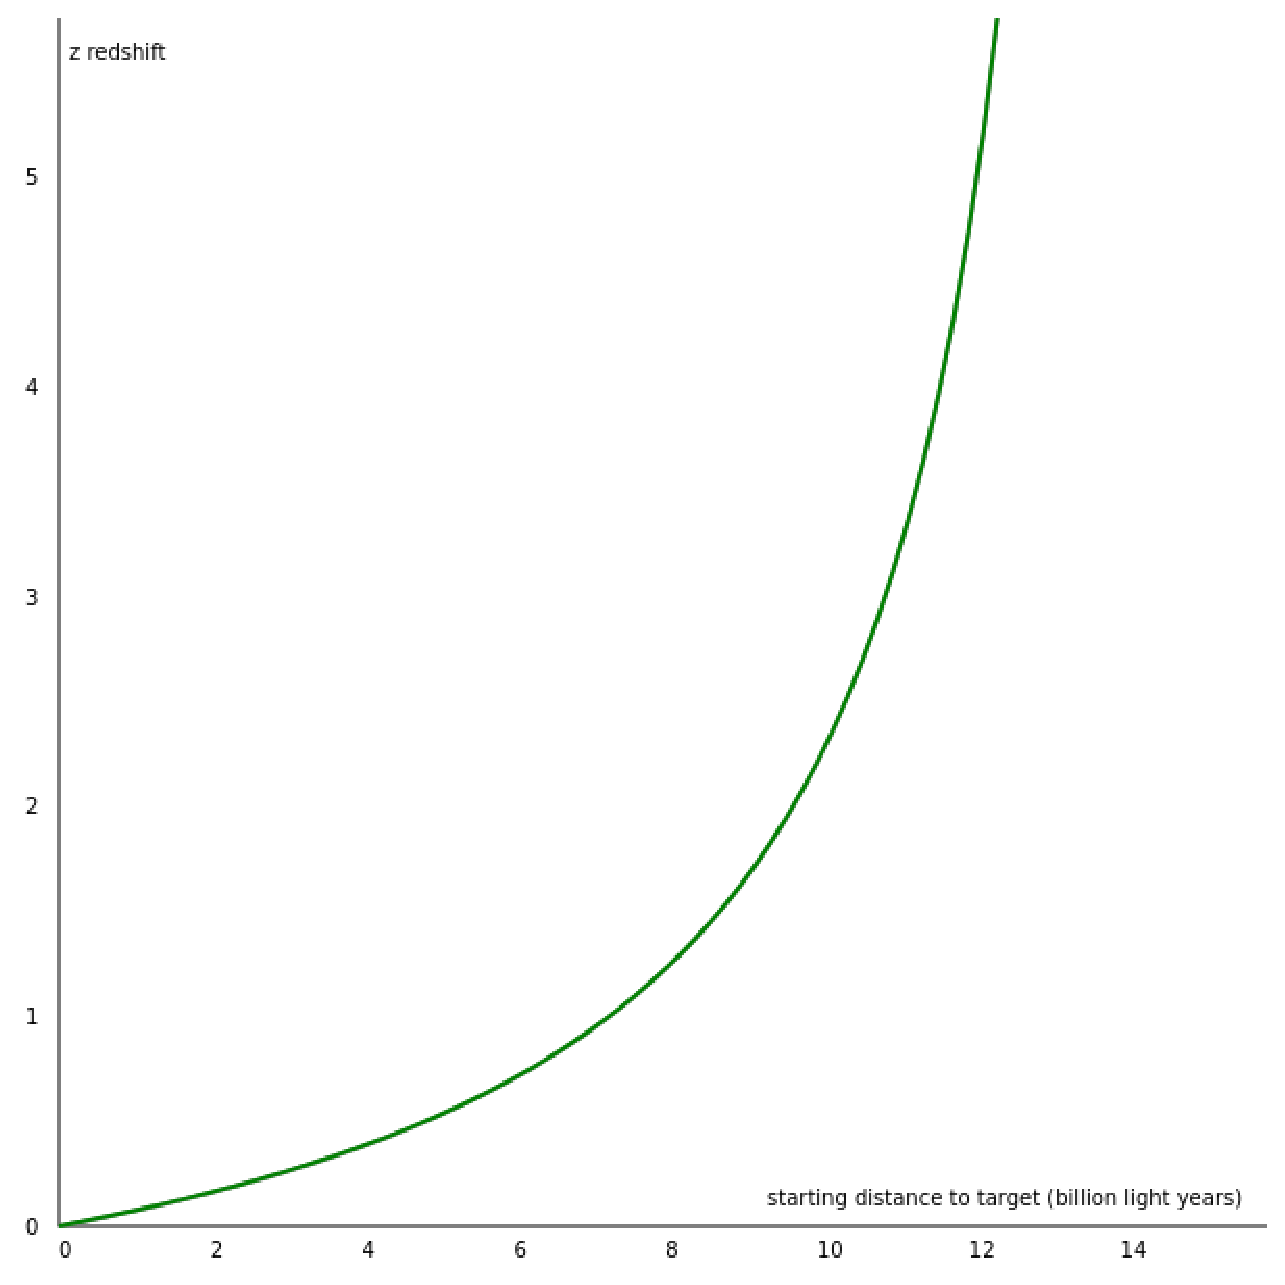
\includegraphics[width=2.0in]{graph_white_z.eps}}
\vspace*{8pt}
\caption{Hypothesis 1 (green) and expanding models (hidden) produce identical redshifts for distances}
\label{fig:distancez}
\end{figure}

With this data, we can graph z over distance, and we see in Figure 3 that hypothesis 1 (green) covers up the expanding model (hidden) using the same value of $H$. 

This shows that hypothesis 1 predicts identical redshifts for targets of the same distance as the expanding model.
However, they are not identical models; hypothesis 1 predicts the photon reaches the target sooner than the 
photon in the expanding model, as seen in Figure 2. That will be investigated later in this paper.

\subsection{Alternative versions}

Hypothesis 1 is a very straightforward implementation of the principle that a photon's speed decreases with distance. Another possibility is something like an inverse square law:

\begin{equation}
v_{photon} = \frac{c}{1 + (H \times D)^2}
\end{equation}

Hypothesis 2 has some interesting features, but it doesn't match the expected redshift data like hypothesis 1 does. 
You can examine these models and others for yourself at https://mikehelland.github.io/hubbles-law/test.htm.

In these models, the photon shows delays in reaching the targets even though the targets are stationary. The delay occurs because the photon redshifts and its velocity decreases. In such a universe, space is not expanding. 

The remainder of this paper will compare this hypothesis to similar sounding models, discuss the treatment of the photon in the model, and examine possible ways to test the hypothesis.

\section{Comparison to Other Theories}

\subsection{Tired Light}

There have been hundreds of theories that don't involve expanding space trying to explain how light gets "tired" during long intergalactic journeys, starting all the way back in 1929 when the redshift-distance relation was first published.\cite{Reboul} 

Tired light theories fail because they don't account for enough redshift, they can't explain the distance factor, or the redshifts are caused in a way that would include other observable results, which ultimately are not observed.

In general, tired light theories have the following in common:

\begin{itemlist}
 \item Some other phenomenon causes the redshifts 
 \item Light always travels at c, even though it is "tired" 
 \item They are represented by the blue line on the graph, matching a simple static model 
\end{itemlist}

The hypothesis that light's speed is inversely proportional to the distance from its source is different:

\begin{itemlist}
 \item Nothing causes the redshifts, they are as fundamental to nature as inertia 
 \item Light travels at less than c after millions of years 
 \item The time it takes light to reach a target is similar to the expanding model 
\end{itemlist}

In this hypothesis, one could say light does get "tired", but it does so in a way that is conceptually and mathematically unique to the established Tired Light theories.

\subsection{Varying Speed of Light}

For the last few decades there have been versions of a theory going around known as Varying Speed of Light, claiming that the
perceived acceleration of the expansion of the universe can be explained if the speed of light is different now than in the past.\cite{VSL}

In VSL theories:

\begin{itemlist}
 \item c changes 
 \item All photons in the universe slow to the same speed 
 \item Space is expanding 
 \item Intends to represent the accelerating rate of expansion 
\end{itemlist}

The hypothesis in this paper is different:

\begin{itemlist}
 \item c is constant 
 \item Individual photons slow down according to their own history, not the universe's 
 \item Space is not expanding 
 \item Intends to represent cosmological redshift 
\end{itemlist}

The speed of light does vary in this hypothesis, but in a novel way to Varying Speed of Light theories.

\section{Photons}

This model represents light at the individual photon level. It's not a quantum theory, nor is it a relativistic theory, but it's also not completely classical. To illustrate, the photon was defined as having a distance from its source.

\begin{verbatim}
    photon = {
        distance: 0
    }
\end{verbatim}

Where is this photon? It doesn't have an (x,y,z) coordinate. Instead, it occupies every point around its source at the specified distance. It's not a classical particle or wave in this form.

Later, we added velocity, frequency, and wavelength to the photon.

\begin{verbatim}
    photon = {
        distance: 0, 
        velocity: 1, 
        frequency: 6e5, 
        wavelength: 499.65
    }
\end{verbatim}

For the purposes of this model, the photon actually only needs distance and energy.

\begin{verbatim}
    photon = {
        distance: 0, 
        energy: 2.48, 
    }
\end{verbatim}

We know from classical mechanics that the speed of a wave is its frequency $\times$ wavelength. In quantum mechanics the energy of a photon is 
frequency $\times$ Planck's constant ($h$). And hypothesis 1 says the speed of a photon is $c - H \times D.$ Given these formulas:

\begin{equation}
    v_{photon} = c - H \times D
\end{equation}
\begin{equation}
    v_{wave} = f \times w 
\end{equation}
\begin{equation}
    E_{photon} = h \times f 
\end{equation}

the photon's velocity, frequency, and wavelength can be determined at any time from its distance and initial energy. 
However, those values don't need to be there at all times, and since the photon is a quantum particle, they probably shouldn't be there until we need them.
What we know about a photon we determine from its interaction with a measurement apparatus, not because we can observe it in-flight.

We know that a redshifted photon will deliver less energy than it started out with. 
Assuming the ratio of energy observed to energy emitted is the same ratio as the photon's velocity to $c$:

\begin{equation}
E_{observed} = E_{emitted} \times \frac{v}{c} 
\end{equation}

then using hypothesis 1 for $v$ we can calculate the observed energy of a photon using just the photon's original energy and the distance from its source:

\begin{equation}
E_{observed} = E_{emitted} \times \frac{c - H\times D}{c}
\end{equation}

\begin{equation}
E_{observed} = E_{emitted} \times (1 - \frac{H\times D}{c})
\end{equation}

The photon's distance from where it was emitted is crucial to keep in mind at all times. Consider light that has traveled billions of years to reach your telescope. The light enters the lens, gets focused to the eyepiece, and then into your eyeball.

That seems pretty straightforward, but at some level, some type of interaction with the light and the lens must be focusing the light. At the quantum level, the photon will have been absorbed by atoms in the lens. Then it is re-emitted (or an entirely new photon is emitted), and focused to your telescope's eyepiece.
The photon may have traveled great distances from its source before it encountered your telescope, but the light inside the telescope will be very close to its source: the lens that focused it. The distance to the source of the photons in the telescope will be less than a meter, not millions of light years.

In that case the refreshed photon will be traveling at c, which now results in an elongated wavelength when calculated.

\section{Tests}

\subsection{Measure the speed of a cosmologically redshifted photon}

This is the first obvious test of the hypothesis. But it would take thousands or millions of years to perform a fully controlled experiment where light is emitted with a known energy at a known time and travels across a known distance to see the effects of redshift.
Using light that has already traveled millions of years seems to be the only choice. But interacting with the photon will cause it to reset its distance and speed, as mentioned in the previous section. The task then is to come up with a clever way to measure the speed of ancient light without disturbing the photon. 

Consider a long tube in space with a telescope at one end and an open shutter at the other, as pictured in Figure 4. 
The telescope has a nearby galaxy and a highly redshifted galaxy in its sight. 

\begin{figure}[h]
\centerline{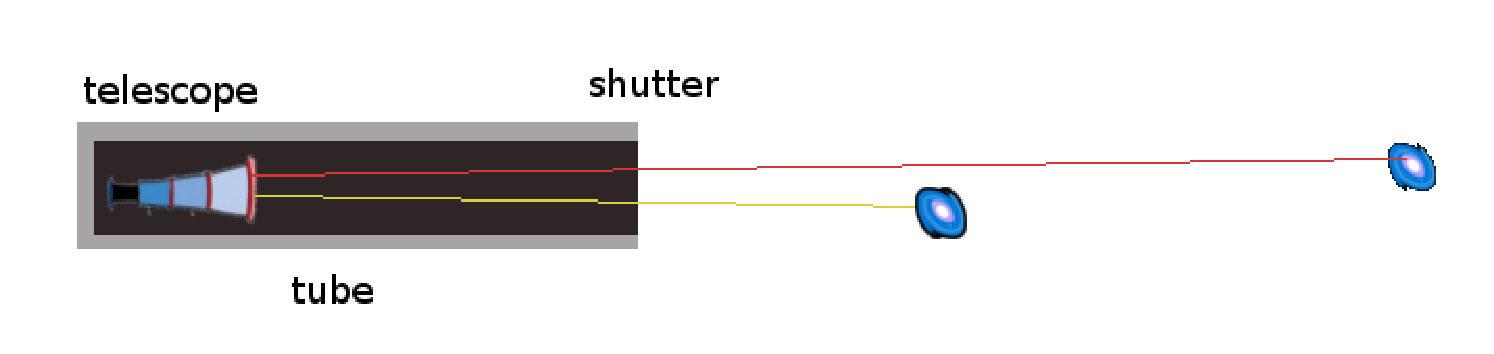
\includegraphics[width=5.0in]{experiment1.eps}}
\vspace*{8pt}
\caption{If redshifted light is traveling slower, it should disappear last from the telescope's view when the shutter is closed}
\label{fig:experiement}
\end{figure}

What happens when the shutter is closed?

\textbf{Prediction: }Because the red light is moving slower than the yellow light, first the nearby galaxy will disappear from view, then the distant one.

Obviously the longer the tube is the better the experiment would be. The tube also isn't completely necessary, if another distant craft could act as the shutter.
 If we use a predictable and fast enough natural object in space as the shutter, that might work too. The shutter must not reflect any light. 
 The moon is too bright and too slow to work.

\subsection{Test 2: the time to target discrepancy}

It was noted earlier that the expanding model and hypothesis 1 produce the same redshifts for the same value of H for the same distances, but at different times. 
The photon in hypothesis 1 reaches its targets in less time than the photon in the expanding model, as can be seen in Figure 2.

To look at this further, WolframAlpha was used to get the expected lookback time and co-moving distance for objects with a z of 1 through 25,
and values of 74 km/s/Mpc and 64.7 km/s/Mpc for Hubble's constant, which is listed in Table 1.


\begin{table}[p]
\tbl{Expected z, lookback time, and co-moving distance for $H_{0}=74$ km/s/Mpc and $H_{0}=67.4$ km/s/Mpc of the standard model using WolframAlpha}
{\begin{tabular}{c@{\qquad}cc@{\qquad}cc}
  \toprule
  \multirow{2}{*}{\raisebox{-\heavyrulewidth}{$z$}} & \multicolumn{2}{c}{$H_{0}=74$} & \multicolumn{2}{c}{$H_{0}=67.4$} \\
  \cmidrule{2-5}
  & Lookback~Time & Co-moving~Distance & Lookback~Time & Co-moving~Distance \\
  \midrule
     1    &    7.4   &    10.4   &    8.1   &    11.4 \\ 
     2    &    9.8   &    16.4   &   10.8   &    18.0 \\ 
     3    &   11.0   &    20.1   &   12.1   &    22.1 \\ 
     4    &   11.6   &    22.8   &   12.7   &    25.0 \\ 
     5    &   11.9   &    24.7   &   13.1   &    27.1 \\ 
     6    &   12.2   &    26.2   &   13.4   &    28.8 \\ 
     7    &   12.3   &    27.5   &   13.5   &    30.2 \\ 
     8    &   12.4   &    28.5   &   13.7   &    31.3 \\ 
     9    &   12.5   &    29.4   &   13.8   &    32.2 \\ 
    10    &   12.6   &    30.1   &   13.8   &    33.0 \\ 
    11    &   12.7   &    30.7   &   13.9   &    33.8 \\ 
    12    &   12.7   &    31.3   &   14.0   &    34.4 \\ 
    13    &   12.7   &    31.8   &   14.0   &    34.9 \\ 
    14    &   12.8   &    32.3   &   14.0   &    35.4 \\ 
    15    &   12.8   &    32.7   &   14.1   &    35.9 \\ 
    16    &   12.8   &    33.1   &   14.1   &    36.3 \\ 
    17    &   12.8   &    33.4   &   14.1   &    36.7 \\ 
    18    &   12.9   &    33.7   &   14.1   &    37.0 \\ 
    19    &   12.9   &    34.0   &   14.1   &    37.4 \\ 
    20    &   12.9   &    34.3   &   14.2   &    37.7 \\ 
    21    &   12.9   &    34.6   &   14.2   &    37.9 \\ 
    22    &   12.9   &    34.8   &   14.2   &    38.2 \\ 
    23    &   12.9   &    35.0   &   14.2   &    38.4 \\ 
    24    &   12.9   &    35.2   &   14.2   &    38.7 \\ 
    25    &   12.9   &    35.4   &   14.2   &    38.9 \\  
  \bottomrule
\end{tabular}\label{ta1} }
\end{table}

In the expanding model, the lookback time refers to how long ago the light was emitted, 
and the co-moving distance refers to how far away the light source is now, given that space has expanded since the light was emitted. 

In hypothesis 1, the time it takes to make the journey increases due to the photon slowing down. 
A distant light source won't have moved due to expansion between then and now (though it may have moved due to its own peculiar motion). 
In this case distance and duration trade places. The lookback time correlates with the distance of the target as seen in Figure 5, 
and the co-moving distance correlates with the time it takes to reach the target, as seen in Figure 6.  

\begin{figure}[hb]
\centerline{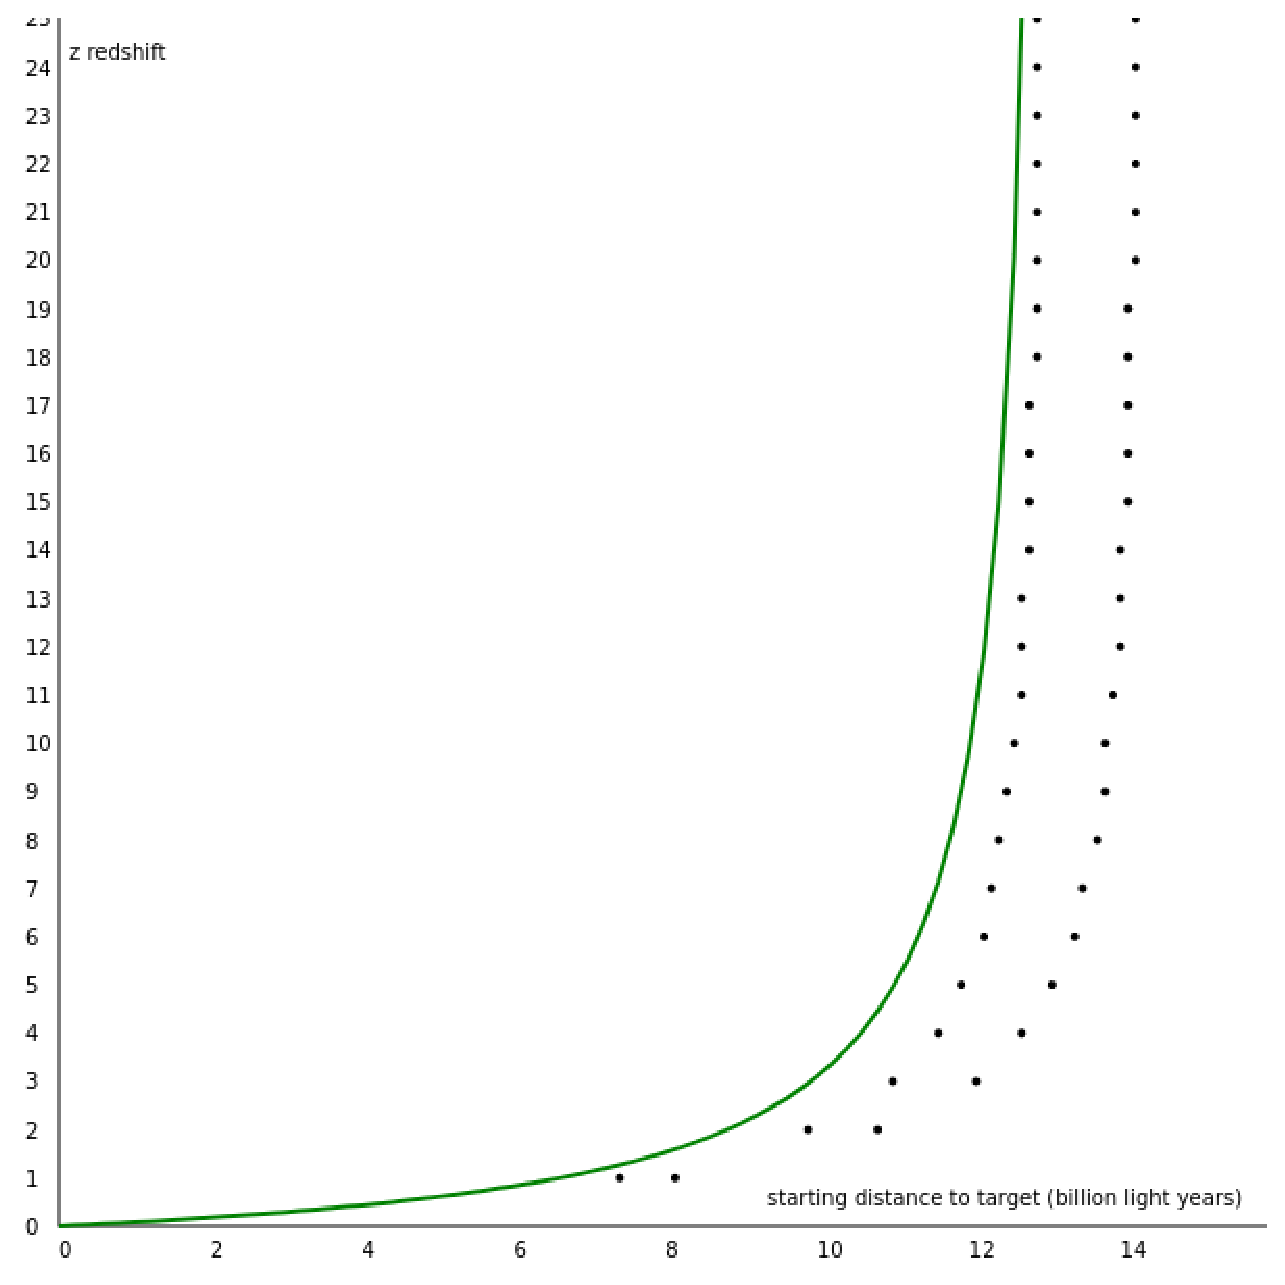
\includegraphics[width=3.0in]{graph_white_test2_2.eps}}
\vspace*{8pt}
\caption{Hypothesis 1 (green line) is a match for lookback times (dots) from Table 1}
\end{figure}

\begin{figure}[hb]
\centerline{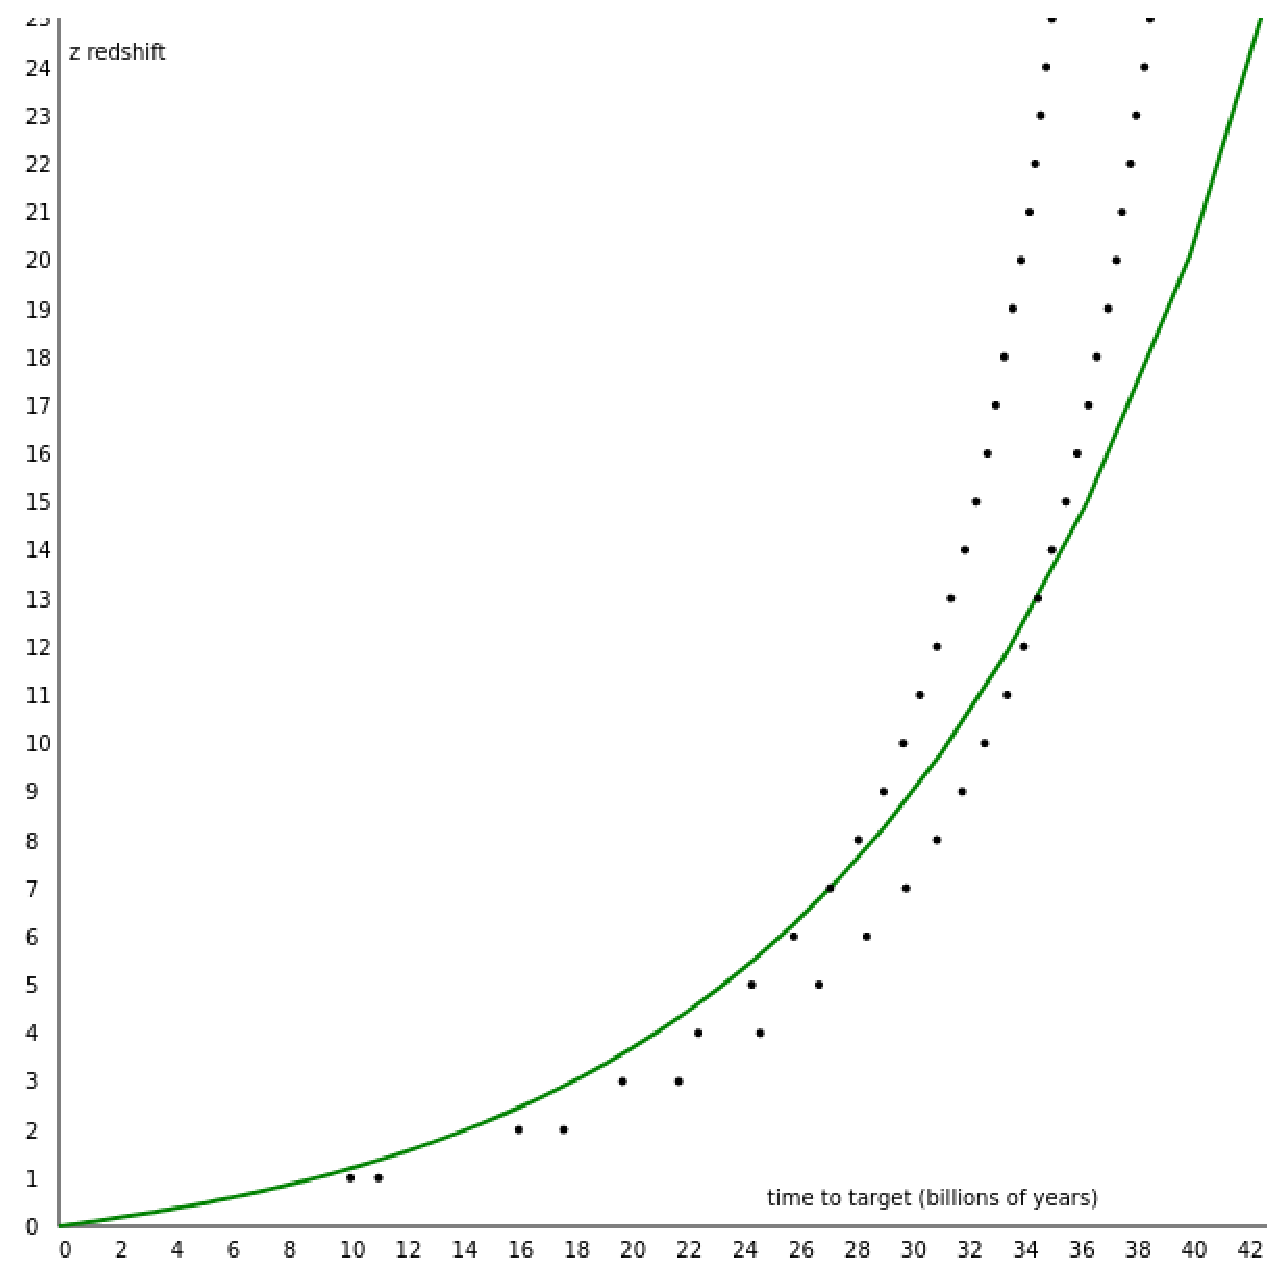
\includegraphics[width=3.0in]{graph_white_test2_3.eps}}
\vspace*{8pt}
\caption{Hypothesis 1 (green line) predicting a lower z for extreme distances than the standard model (dots)\protect\label{fig8}}
\end{figure}

At about a z of 8.0 in Figure 6, hypothesis 1 starts to go off the path of the expanding model, predicting a slower rise in z over time.
This deviation from the standard model appears to be what is measured today and known as the Hubble tension, the difficulty in finding a proper value for Hubble's constant. If hypothesis 1 is adopted as Hubble's Law, the tension is resolved. 

\subsection{Breadcrumbs}

If the photon has less energy when it arrives than when it left, what about the missing energy? If the universe is very old and 
light keeps losing energy, very little would be left of existence by now. 

For this reason, it seems sensible that any energy deducted from the photon during its journey through space might be deposited along its path, like a trail of breadcrumbs. Overtime, this discarded energy could coalesce into something larger. 

This might be supported by observations of walls and filaments of galaxies, although, how that could be made into a quantifiable prediction is presently unclear.

\section{Conclusion}

\begin{quote}
\emph{''We seem to face, as once before in the days of Copernicus, a choice between a small, finite universe, 
and a universe indefinitely large plus a new principle of nature.''} - E. Hubble
\end{quote}


Cosmological redshifts have been a known, observed fact since 1929.
We could assume the redshifts indicate motion, which means 
the universe is expanding, 
there are age and size limits to the universe, 
the universe inflated in the first nanosecond, 
it is dominated by dark matter and dark energy, 
and it's currently accelerating.

Or we could assume the redshifts are themselves a new feature of the universe, which means
light doesn't travel to infinity at a constant speed,  
and what we observe is an insignificant sample of a universe that stretches indefinitely in time and space. 


When interpreting the redshifts as Doppler effects in the 20th century, astronomers didn't know this idea would lead to inflation or dark energy. In fact, they chose the velocity-shift interpretation because it was known and familiar and didn't require new laws of physics.
In retrospect, it should come as no surprise to us that when telescopes could show us what's beyond the Milky Way, they would also reveal a new fundamental law of nature.

If dark energy is in the consideration as a possible fundamental ingredient of nature despite having never been observed, then the actual observations that led to its conjecture, cosmological redshift, should be considered as well.


\begin{thebibliography}{0}


\bibitem{Riess} A. G. Riess et al. [Supernova Search Team], {\it  Astron. J.}, 116, 1009 (1998).

\bibitem{Planck} N. Aghanim et al., {\it“Planck 2018 results. VI. Cosmological parameters},
(2018)

\bibitem{Hubble} E. Hubble, in {\it The Observational Approach to Cosmology}, 22, (1937)

\bibitem{Reboul} H.J. Reboul, {\it Astron. Astrophys. Supp. Ser.} {\bf 45},
129--144 (1981).

\bibitem{VSL} J. Magueijo, {\it Reports on Progress in Physics}, Vol. 66, Iss. 11, 2025-2068 (2003).

\end{thebibliography}
\end{document}